\chapter{Réalisation}
% l’ordre de présentation le plus logique est souvent l’ordre chronologique dans lequel les tâches ont été accomplies. Il faut présenter les points forts en distinguant nettement l’existant et la plus-value apportée par le stagiaire. Si des solutions ont été envisagées, mais non retenues, il peut être intéressant de les présenter en expliquant pourquoi elles ont été abandonnées. C’est toute la chaîne, de la prise de connaissance du problème à la solution apportée, qui doit être déroulée.

% Cette partie débouche nécessairement sur des résultats qu’il faut énoncer en précisant leurs exploitations actuelles ou à venir. Il faut annoncer clairement ce qui a été réalisé ou non par rapport à la mission de départ. Cette partie peut être complétée par des propositions personnelles du stagiaire pour prolonger son travail, et même par des critiques positives de son environnement de travail.

% Tentative plan
%5.1. recherche doc
%5.2. patch "reimplement"
%5.3. build "growing"
%5.4. optimise "growing"
%5.5. conclusions on "growing" and "awd"

\section{Recherche documentaire}
La première partie du projet, qui à durée à peu près une semaine, à été la recherche documentaire et la prise en main des outils.
Ce travail à été effectué à partir des documents fournis par notre maître de stage, de la documentation de \gls{pytorch}\autocite{60MinBlitzTorch,ByExampleTorch,Classify,doc_pytorch} et de \gls{g5k}, complétés par nos recherches personnelles.
%TODO cite articles fournis
%TODO cite g5k doc
%TODO cite recherches personnelle

%-> liste de ref bib%\clearpage % lib, tutos, concepts
\section{Étude et ré-implémentation simplifiée du modèle \gls{soa}}
\subsection{Travail effectué}\label{subsec:codebase}
La deuxième partie du projet à été la prise en main de la base de code fournie.
Il s'agit d'une implémentation \gls{soa} d'un \gls{lm} au niveau du caractère, sur laquelle notre maître de stage avait commencé à travailler.
Le code d'origine provient du dépôt \og awd-lstm-lm\fg{}\autocite{awd_source}, qui contenait un modèle \gls{soa} de \gls{lm} au niveau du caractère.

Au début du stage, la base de code contenait~:
\begin{itemize}
	\item la version d'origine du dépôt~;
	\item un début de ré-implémentation simplifiée du \gls{model} de la version d'origine~; cette version  devait servir de base pour développer le \gls{model} du \gls{gmsnn}, ainsi que de comparaison pour les performances du nouveau \gls{model}~; elle comportait quelques \glspl{bug} et ne fonctionnait pas en l'état~;
	\item un début de travail sur l'architecture du \gls{gmsnn}.
\end{itemize}

\vspace{1em}
L'objectif de cette étape était de faire fonctionner la ré-implémentation simplifiée du \gls{model}.

Pour cela, nous avons déchiffré et re-documenté le code, qui contenait des fragments obsolètes et peu documentés.
Après le déchiffrage, il à fallu comprendre et réparer les fragments défectueux.

\subsection[\Glsentrytext{model} ré-implémenté simplifiée]{\Gls{model} ré-implémenté simplifiée}
Le \gls{model} simplifiée produit est composé d'un module encodant les caractères, d'un \gls{rnn} particulier (un \gls{lstm}, voir \autoref{def:lstm}), et d'un module produisant une distribution de probabilité sur les caractères connus. La \autoref{fig:reimplement} représente cette architecture.

\begin{figure}[h]
	\centering
	\scalebox{1}{\usetikzlibrary{calc}
\newsavebox\mydictbox
\savebox\mydictbox{%
  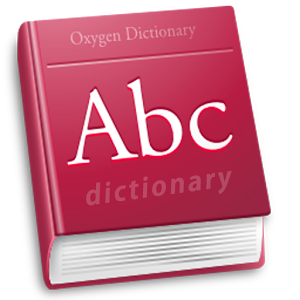
\includegraphics[width=3em]{/home/emarquer/InternshipSynalp2018/report_internship/images/tool_translate_offline_dictionary.png}
}

\begin{tikzpicture}[shorten >=2pt,->,draw=black, node distance=7em]
    \tikzstyle{every pin edge}=[<-,shorten <=2pt]
	\tikzstyle{module}=[minimum size=3em, fill=gray!50!]
	\tikzstyle{char}=[module, circle, fill=green!50!]%, label={below:\usebox\mydictbox}]
	\tikzstyle{text label}=[rectangle, text centered, text width=7em, node distance=5em]
	\tikzstyle{nn}=[rectangle, module, fill=orange!50!]
	\tikzstyle{rnn}=[nn, fill=red!50!]

	\node[char] (char) {\$};
	\node[nn, right of=char] (emb) {Emb.};
	\node[rnn, right of=emb] (rnn) {LSTM};
	\draw[->] (rnn.north) to [out=90,in=90, looseness=2] ($(rnn.west) + (-0.5,0)$) to [out=-90,in=-90, looseness=2] (rnn.south);
	\node[nn, right of=rnn] (lin) {Lin.};
	\node[char, right of=lin] (out) {P(\$$_{+1}$)};
	\draw[->] (char) to (emb);
	\draw[->] (emb) to (rnn);
	\draw[->] (rnn) to (lin);
	\draw[->] (lin) to (out);
	%\node[char] (char) {\$};


    \node[text label, above of=char] (charl) {Caract\`{e}re};
    \node[text label, above of=emb] (embl) {Encodage du caract\`{e}re};
    \node[text label, above of=rnn] (rnnl) {RNN};
    \node[text label, above of=lin] (linl) {Transformation en distribution de probabilit\'{e}};
    \node[text label, above of=out] (outl) {Probabilit\'{e} d'apparition des caract\`{e}res};
\end{tikzpicture}}
	\caption[Architecture du \glsentrytext{model} réimplémenté]{Architecture du \gls{model} réimplémenté. Le modèle prend en entrée des caractères, et produit des probabilités sur quel caractère apparaîtra ensuite.}\label{fig:reimplement}
\end{figure}

Le module d'encodage des caractères, appelé \foreign{embeding layer} en anglais (littéralement \og couche d'inclusion\fg{}), produit une représentation apprise de chaque caractère sous forme de \gls{tensor}. Ce \gls{tensor} est appelé \gls{embedding}. Ce module, entraîné, peut apprendre des propriétés spécifiques à chaque caractère. Par exemple ce module peut apprendre que telle lettre est une consonne et que telle autre est un caractère de ponctuation. \label{def:embeding}

Le \gls{rnn} traite les caractères sous forme de séquence, et peut ainsi apprendre la structure en mots, la syntaxe et d'autres propriétés du langage.

Le module produisant la distribution de probabilité est un module linéaire.
Il transforme les informations produites par le réseau de neurones en probabilité pour chaque caractère d'être le prochain caractère de la séquence. % TODO def module linéaire

Voir les annexes \ref{subsec:testreimp_1}, \ref{subsec:testreimp_2} et \ref{subsec:testreimp_3} pour les rapports sur le \gls{model} ré-implémenté. 

\subsection{Conclusion}
Cette étape, outre la préparation du code, à permit la mise en œuvre et une meilleur compréhension des concepts appris durant l’étape précédente. C'est la première pierre de l'édifice qu'est le \gls{gmsnn}.\clearpage % reprise sur de l'existant, découverte de la lib
\section{Implémentation du nouveau modèle}
\subsection{Travail effectué}\label{def:lstm_2}
La troisième partie du projet a été la réalisation d'un prototype de l'architecture \gls{gmsnn}, basé sur la ré-implémentation simplifiée du \gls{model} \gls{soa}.

L'architecture du \gls{gmsnn} est celle du \gls{model} ré-implémenté, mais le \gls{rnn} y est remplacé par le \gls{module_gmsnn} (voir figure \ref{fig:reimplement_gmsnn}, \autopageref{fig:reimplement_gmsnn}). C'est sur ce nouveau \gls{module_gmsnn} que le reste du travail au cours du \gls{project_gmsnn} a été effectué.

De la même façon qu'avec la version ré-implémentée, le modèle prend en entrée des caractères, et produit des probabilités sur le caractère qui apparaîtra ensuite.

Ce prototype a permis de mettre en place les mécanismes de base du modèle.

Durant cette étape, nous avons mis en place l'architecture multi-échelle avec deux mécanismes fondamentaux, la transmission de l'information d'une échelle à l'autre et l'agrégation de l'information de toutes les échelles.

Chaque échelle qui compose le \gls{module_gmsnn} est un \gls{lstm}, qui est le \gls{rnn} utilisé dans le \gls{model} d'origine.

\begin{figure}[ht]
	\centering
	\scalebox{1}{\usetikzlibrary{calc}

\begin{tikzpicture}[shorten >=2pt,->,draw=black, node distance=7em]
    \tikzstyle{every pin edge}=[<-,shorten <=2pt]
	\tikzstyle{module}=[minimum size=3em, fill=gray!50!]
	\tikzstyle{char}=[module, circle, fill=green!50!]%, label={below:\usebox\mydictbox}]
	\tikzstyle{text label}=[rectangle, text centered, text width=7em, node distance=5em]
	\tikzstyle{nn}=[rectangle, module, fill=orange!50!]
	\tikzstyle{rnn}=[nn, fill=red!50!]

	\node[char] (char) {\$};
	\node[nn, right of=char] (emb) {Emb};
	\node[rnn, right of=emb] (rnn) {GMSNN};
	\draw[->] (rnn.north) to [out=90,in=90, looseness=2] ($(rnn.west) + (-0.5,0)$) to [out=-90,in=-90, looseness=2] (rnn.south);
	\node[nn, right of=rnn] (lin) {Lin};
	\node[char, right of=lin] (out) {P(\$$_{+1}$)};
	\draw[->] (char) to (emb);
	\draw[->] (emb) to (rnn);
	\draw[->] (rnn) to (lin);
	\draw[->] (lin) to (out);
	%\node[char] (char) {\$};


    \node[text label, above of=char] (charl) {Caract\`{e}re};
    \node[text label, above of=emb] (embl) {Encodage du caract\`{e}re};
    \node[text label, above of=rnn] (rnnl) {RNN};
    \node[text label, above of=lin] (linl) {Transformation en distribution de probabilit\'{e}};
    \node[text label, above of=out] (outl) {Probabilit\'{e} d'apparition des caract\`{e}res};
\end{tikzpicture}}
	\caption[Architecture du \glsentrytext{model} GMSNN]{Architecture du \glsentrytext{model} GMSNN}\label{fig:reimplement_gmsnn}
\end{figure} 

\pagebreak
\subsection{Transmission de l'information}
Pour rappel, la transmission de l'information se fait d'une couche donnée à la couche immédiatement supérieure.
Cette transmission se fait périodiquement, en fonction d'un nombre appelé fréquence de transmission.

%Par exemple, pour fréquence de transmission de $3$~: 
%\begin{itemize}
%	\item toutes les $3$ entrées de la couche $n-1$, la couche $n$ reçoit de l'information de la couche $n-1$~;
%	\item toutes les $3$ entrées de la couche $n$ (soit toutes les $3^2$ entrées de la couche $n-1$), la couche $n+1$ reçoit de l'information de la couche $n$.
%\end{itemize}
%\vspace{1em}

Dans un premier temps, il a fallu choisir quelle information transmettre d'une échelle à l'échelle supérieure. En effet, les \glspl{rnn} produisent à la fois une sortie et un \gls{tensor} contenant leur mémoire. L'utilisation de l'\gls{embedding} a été écartée initialement, car elle n'est pas en accord avec le principe d'abstraction de l'architecture proposée.

%\pagebreak
Le choix s'est porté sur le \gls{tensor} contenant la mémoire, qui contient donc les informations abstraites par l'échelle, contrairement à la sortie qui  contient uniquement les informations pour prédire le caractère suivant.

%\begin{figure}[h]
%	\begin{subfigure}{0.45\textwidth}
%		\centering
%%		\scalebox{1}{\usetikzlibrary{calc}

\begin{tikzpicture}[shorten >=2pt,->,draw=black!50, node distance=7em]
    \tikzstyle{every pin edge}=[<-,shorten <=2pt]
	\tikzstyle{module}=[minimum size=3em, fill=gray!50!]
	\tikzstyle{char}=[module, circle, fill=green!50!]
	\tikzstyle{text label}=[rectangle, text centered, text width=7.5em, node distance=7em]
	\tikzstyle{nn}=[rectangle, module, fill=orange!50!]
	\tikzstyle{rnn}=[nn, fill=red!50!]

	\node[rnn, pin={[pin edge={<-}, pin distance=3em]south:Entr\'{e}e}] (rnn1) {RNN};
	\node[rnn, above of=rnn1] (rnn2) {RNN};
	\node[rnn, above of=rnn2, pin={[pin edge={->,dashed}, pin distance=3em]north:}] (rnn3) {RNN};

	\foreach \n in {1,...,3}
		\draw[->] (rnn\n.east) to [out=0,in=0, looseness=2] ($(rnn\n.south) + (0,-.5)$) to [out=180,in=180, looseness=2] (rnn\n.west);

	\path[->,dashed] (rnn1)  edge coordinate (@aux) (rnn2);
	\path [late options={name=@aux, pin={[pin edge={-}, text width=10.5em, pin distance=5em]0:Transmission toutes les $n$ entr\'{e}es de l'\'{e}chelle 1}}];
	\path[->,dashed] (rnn2)  edge coordinate (@aux) (rnn3);
	\path [late options={name=@aux, pin={[pin edge={-}, text width=10.5em, pin distance=5em]0:Transmission toutes les $n$ entr\'{e}es de l'\'{e}chelle 2}}];

	\foreach \n in {1,...,3}
	    \node[text label, left of=rnn\n] (rnn\n l) {\'{E}chelle \n};
	\node[right of=rnn3, node distance=10.7em, text width=11em, yshift=3em] (rnn l) {$n$ est la fr\'{e}quence de transmission};
\end{tikzpicture}}
%		\caption{Architecture en blocs simples}
%	\end{subfigure}
%	\begin{subfigure}{0.45\textwidth}
%		\centering
%%		\scalebox{1}{\input{plots/base_gmsnn_unfolded}}
%		\caption{Architecture en blocs dépliés}
%	\end{subfigure} 
%	\caption[Architecture fondamentale du \glsentrytext{gmsnn}]{Architecture fondamentale de \gls{module_gmsnn}}\label{fig:module_gmsnn_base}
%\end{figure}

L'annexe \ref{subsec:testms} (\autopageref{subsec:testms}) présente le rapport sur le prototype. \clearpage % reprise sur de l'existant
\section{Intégration de systèmes de visualisation}\label{sec:gmsnn_track}
Afin d'évaluer les performances du modèle dans la suite du projet, il à été nécessaire d'établir un système de visualisation des performances.

\subsection{Utilisation de librairies}
Dans un premier temps, diverses librairies permettant de visualiser l'état du \gls{nn} ont étés testées, en particulier VisualDL \autocite{VisualDLGit,VisualDLSite}.

Malheureusement, aucune de ces librairies ne sont pas en mesure de supporter les architectures les plus complexes (en particulier celles qui impliquent des \gls{rnn}).

Ainsi, aucune des librairies testées n'a fonctionné avec notre modèle.

\subsection{Création d'un outil personnalisé}
Nous avons donc réalisé un module capable d'enregistrer des données et de réaliser des graphiques. Nous nous sommes basés sur le module \og matplotlib\fg{}\autocite{matplotlib} de Python, et sur une variante française du format CSV\autocite{csv}.

Ce module à évolué tout au long du projet pour s'adapter à nos besoins.

L'intégralité des graphiques produits dans les divers rapports du projet (disponibles en annexes) à été produit avec ce module.
\clearpage % reprise sur de l'existant
\section{Optimisation et amélioration du nouveau modèle}
%opti 1
	%addcat
	%reprise train
	%batch
%pb mémoire (beaucoup d'opti perf nécessite d'augmenter la taille des params/modules/tenseurs...) & tps (la plupart des otpis perfs augmentent le tps de calcul nécessaire, et de base le modele naif est trop lent)
%pb memoire réglé, tentative infructueuse d'améliorer les perfs avec améliorations préparées en parallèle
	%+ params
	%lbl
% ccl plus pb mémoire & tps, opti z'oignons (XD) même, 5 min c'est balèze

Une fois le prototype fonctionnel, nous avons amélioré ses performances.
Par performances, nous entendons principalement le temps nécessaire pour que la qualité prédictive du modèle dépasse un certain seuil.

Pour améliorer ce temps d'entraînement, il est possible de travailler sur deux dimensions~:
\begin{itemize}
	\item la \emph{quantité de \glspl{data}} traitées en un laps de temps~;
	pour cela on peut optimiser les algorithmes et le modèle pour réduire le temps nécessaire pour traiter les \glspl{example}~;
	c'est une \emph{stratégie quantitative}~;
	\item la \emph{qualité} de l'apprentissage pour une quantité fixée de \glspl{data}~;
	pour cela on peut améliorer le modèle en modulant les paramètres (comme la fréquence de transmission) ou en implémentant de nouvelles mécaniques~;
	c'est une \emph{stratégie qualitative}.
\end{itemize}

Les deux stratégies ont été utilisées. Il faut noter que certaines améliorations qualitatives ont un impact quantitatif négatif.

Principalement, le travail effectué pendant cette partie du projet est un travail de débogage, d'analyse et d'optimisation, avec peu d'implémentation de nouvelles mécaniques dans le \gls{model}.

\subsection[Agrégation des sorties des couches]{Agrégation des sorties des couches~: d'une stratégie additive à une concaténation}\label{subsec:addcat_}
La première optimisation a été de changer la façon de regrouper les informations de toutes les \og échelles\fg{} avant de les transmettre au module produisant la distribution de probabilité.

Initialement, les sorties de toutes les \og échelles\fg{} étaient sommées. Cela permettait de maintenir des \glspl{tensor} de dimensions uniformes quel que soit le nombre d'\og échelle\fg{} (voir figure \ref{fig:add}, \autopageref{fig:add}).

Après discussion avec le maître de stage, la stratégie d'agrégation à été changé en une concaténation des sorties.

Comme montré dans la figure \ref{fig:cat} (\autopageref{fig:cat}), les sorties sont mises côte-à-côte afin de former un nouveau \gls{tensor} et la taille du \gls{tensor} concaténé change en fonction du nombre d'entrées.
La manipulation de \glspl{tensor} de taille non fixée est très ardue dans ce cas précis, bien que nous ne développerons pas plus avant les raisons de cette difficulté.

Cela a nécessité l'abandon de la propriété de croissance à l'infini de l'architecture (décrite \autoref{inf_growth}, \autopageref{inf_growth}), au profit d'un nombre maximal d'échelles défini à l'avance ou déterminée à l'aide d'une formule en fonction des données disponibles (décrite \mbox{\autoref{growth_formula}}, \autopageref{growth_formula}).

\begin{figure}[ht]
	\begin{subfigure}{0.45\textwidth}
		\centering
		\scalebox{1}{\def\layersep{5em}
\begin{tikzpicture}[shorten >=1pt,->,draw=black, node distance=\layersep]
\tikzstyle{every pin edge}=[<-,shorten <=1pt]
\tikzstyle{block}=[minimum size=2em];
\tikzstyle{value}=[rectangle, fill=green!50,block];
\tikzstyle{operation}=[block, circle,inner sep=0pt, fill=red!50];
\tikzstyle{nonlinearity}=[rectangle,block, fill=blue!50];
\tikzstyle{annot} = [text width=6em, text centered]

% Draw the input layer nodes
\foreach \name / \y in {1,...,3}
% This is the same as writing \foreach \name / \y in {1/1,2/2,3/3,4/4}
\node[value, label={[]north:{\'{E}chelle \y}}] (I-\name) at (0,-2*\y) {\y};
\node[value, label={[]north:{\'{E}chelle 4}}, opacity=.5] (I-4) at (0,-8) {4};

% Draw the output layer node
\node[operation, right of=I-2] (ope) {{\Large +}};
\node[value, right of=ope, label={[]north:$1+2+3+4$}](cat){};
% Draw the output layer node
%\node[nonlinearity, right of=cat] (lin) {Lin};
%\node[annot, right of=lin, text width=7em,xshift=2em ] (out) {Distribution de probabilit\'{e}s};

% Connect every node in the input layer with every node in the
% hidden layer.
\foreach \source in {1,...,3}
\path (I-\source.east) edge (ope);
\path (I-4.east) edge[dashed, opacity=.5] (ope);
\path (ope) edge (cat);
%\path (cat) edge (lin);
%\path (lin) edge (out);
\end{tikzpicture}}
		\caption[Stratégie d'agrégation additive]{Stratégie d'agrégation additive}\label{fig:add}
	\end{subfigure}
	\begin{subfigure}{0.45\textwidth}
		\centering
		\scalebox{1}{\def\layersep{5em}
\begin{tikzpicture}[shorten >=1pt,->,draw=black, node distance=\layersep]
    \tikzstyle{every pin edge}=[<-,shorten <=1pt]
    \tikzstyle{block}=[minimum size=2em];
    \tikzstyle{value}=[rectangle, fill=green!50,block];
    \tikzstyle{operation}=[block, circle,inner sep=0pt, fill=red!50];
    \tikzstyle{nonlinearity}=[rectangle,block, fill=blue!50];
    \tikzstyle{annot} = [text width=6em, text centered]

    % Draw the input layer nodes
    \foreach \name / \y in {1,...,3}
    % This is the same as writing \foreach \name / \y in {1/1,2/2,3/3,4/4}
        \node[value, label={[]north:{\'{E}chelle \y}}] (I-\name) at (0,-2*\y) {\y};
	\node[value, label={[]north:{\'{E}chelle 4}}, opacity=.5] (I-4) at (0,-8) {4};

    % Draw the output layer node
    \node[operation, right of=I-2] (ope) {Cat};
    \node[value, right of=ope](cat){2};
    \node[value, above of=cat, node distance=2.1em]{1};
    \node[value, below of=cat, node distance=2.1em](3){3};
    \node[value, below of=3, node distance=2.1em, opacity=.5]{4};
    % Draw the output layer node
    \node[nonlinearity, right of=cat] (lin) {Lin};
	\node[annot, right of=lin, text width=7em,xshift=2em ] (out) {Distribution de probabilit\'{e}s};

    % Connect every node in the input layer with every node in the
    % hidden layer.
    \foreach \source in {1,...,3}
        \path (I-\source.east) edge (ope);
	\path (I-4.east) edge[dashed, opacity=.5] (ope);
	\path (ope) edge (cat);
	\path (cat) edge (lin);
	\path (lin) edge (out);
\end{tikzpicture}}
		\caption[Stratégie d'agrégation par concaténation]{Stratégie d'agrégation par concaténation}\label{fig:cat}
	\end{subfigure} 
	\caption{Stratégies d'agrégation}
\end{figure}

La stratégie par concaténation est plus lente en terme de temps de calcul que la stratégie additive, cependant pour le même temps de calcul elle permet d'obtenir de meilleurs résultats. La figure \ref{fig:addcat} (\autopageref{fig:addcat}) représente ces résultats. Le temps de calcul alloué à l'entraînement des deux modèles est identique. Avec la concaténation on entraîne le modèle sur 1/4 des données, avec l'addition on l'entraîne 5 fois sur l'ensemble des données. Avec la concaténation, on obtient un BPC de 3.5, alors qu'on obtient un BPC de 4 avec l'addition.

Plus de détail sur le choix de la stratégie d'agrégation sont disponibles dans l'annexe \ref{subsec:addcat} (\autopageref{subsec:addcat}). 

\begin{figure}[H]
	\centering
	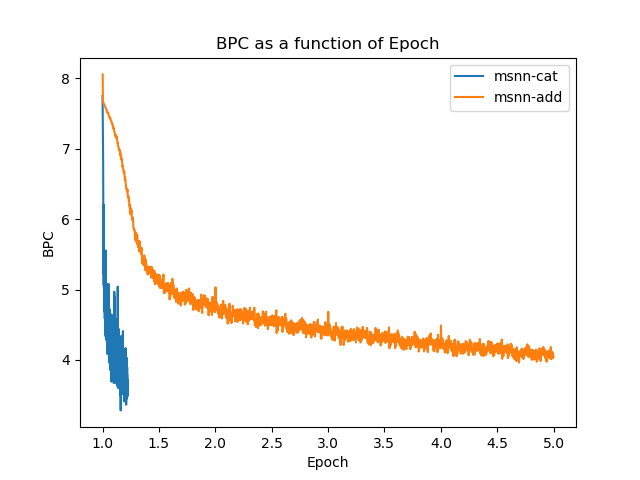
\includegraphics[width=\textwidth]{parts/appendix/reports-gmsnn/docs_esteban-latex/test_reports/comparative-bpc-msnn-det-msnn-cat.png}
	\caption[Performances comparées des stratégies additive et par concaténation]{Performances comparées des stratégies par concaténation \textit{(msnn-cat)} et additive \textit{(msnn-add)}}\label{fig:addcat}
\end{figure} % new
\subsection{Sauvegarde, interruption et reprise de l'entraînement}\label{subsec:gmsnn_save}
Une fonctionnalité s'est très vite détachée comme essentielle~: la sauvegarde du \gls{model}, et l'interruption et la reprise de l'entraînement.

En effet, avec des entraînements très lents et donc longs, il était nécessaire de pouvoir suspendre l'entraînement afin de répartir le temps d'entraînement sur plusieurs sessions de plusieurs heures. De plus, les sauvegardes permettaient de conserver le modèle une fois qu'il est entraîné.

Le système implémenté permet d'effectuer cycliquement des sauvegarde du modèle ainsi que de l'état de l'entraînement, permettant ainsi une reprise en l'état de l'entraînement.

Pour la réalisation du système, le principal obstacle à été le malfonctionnement initial des outils fournis par \gls{pytorch}.
Cela à poussé à la conception d'un système de sauvegarde personnalisé mais malheureusement assez complexe.
Cependant, la mise-à-jour majeure de la librairie qui c'est déroulé à point nommé à résolu le problème, et c'est avec les outils de \gls{pytorch} que le système de sauvegarde à finalement été implémenté.

Voir l'annexe \ref{subsec:save} pour un rapport contenant plus de détail sur le système de sauvegarde. % new
\subsection{Tentatives d'optimisation, fuites de mémoire et lenteur de l'entraînement}\label{subsec:optimem}

Les optimisations testées par la suite ont révélé des fuites de mémoire et mis en lumière une lenteur excessive de l'apprentissage.

Les optimisations en question ont été suspendues le temps de la résolution de ces deux problèmes.
Il s'agit de~:
\begin{itemize}
	\item l'utilisation de \glspl{batch} simultanés (voir \autoref{subsec:optibatch}, \autopageref{subsec:optibatch})~; 
	\item l'augmentation du nombre de \glspl{parameter} du \gls{model} (voir \autoref{subsec:optiparam}, \autopageref{subsec:optiparam})~;
\end{itemize}

%\hspace{1em}
\subsubsection{Consommation de mémoire et de temps de calcul accrue}
Un effet direct des optimisations testées est l'augmentation de la consommation de mémoire.

Cette consommation accrue a causé le plantage\footnote{Un plantage en informatique est l'arrêt d'un programme causé par un dysfonctionnement.} de plusieurs tests, révélant la présence de fuites critiques de mémoire.
Un ralentissement progressif de l'entraînement a aussi été mis en évidence pendant l'analyse du problème.
Le plus surprenant a été la corrélation forte observée entre le temps de calcul et la consommation de mémoire.

Un premier correctif a fourni une amélioration notable mais insuffisante.
Il remplaçait le \gls{lstm} de chaque couche (voir \autoref{def:lstm_2}, \autopageref{def:lstm_2}) par un \gls{rnn} basique, moins gourmand. Cela permettait aussi d'éliminer une redondance entre l'architecture \gls{lstm} et l'architecture \gls{gmsnn}.

\subsubsection{Estimation de la consommation normale du modèle}
La première étape, qui est détaillée dans l'annexe \ref{subsec:memuse} (\autopageref{subsec:memuse}), a été d'estimer l'usage normal de la mémoire (sans fuite), et d'isoler les \glspl{parameter} qui ont le plus d'impact sur la consommation mémoire.
Ceci a confirmé que l'explosion de la consommation n'était pas due à l'architecture en elle-même et qu'il s'agissait bien d'une anomalie dans le fonctionnement du programme.

\subsubsection{Résolution des fuites}
L'analyse et la résolution des fuites de mémoire s'est révélée ardue. Si quelques fuites mineures ont été simples à détecter et réparer, la principale fuite était due à une spécificité non documentée de \gls{pytorch}.

En effet, \gls{pytorch} utilise la \gls{automatic differentiation} pour mettre à jour les \gls{weight} du \gls{nn}.
Pour cela, \gls{pytorch} a besoin de connaître la suite d'opérations et l'implication des différents \glspl{parameter} du \gls{model} et se base sur un \og graphe de computation\fg{}.
C'est le mode de gestion de ce graphe, couplé aux spécificités de l'architecture \gls{gmsnn}, qui est la cause de la principale fuite mémoire.

Le rapport dans l'annexe \ref{subsec:memleak} (\autopageref{subsec:memleak}) présente un extrait de la résolution du problème.

\subsubsection{Conclusion}
Le problème de la fuite de mémoire a été résolu et, avec lui, celui de la lenteur de l'entraînement.
On peut déplorer de ne pas avoir analysé plus en profondeur cet étrange lien entre la mémoire et le temps d'entraînement.
Cependant, la résolution des fuites de mémoire et de la lenteur de l'entraînement était l'objectif principal de cette étape, et l'optimisation du \gls{module_gmsnn} a pu reprendre.

On notera l'ampleur de l'optimisation par rapport à la version initiale~:
\begin{itemize}
	\item le temps de d'entraînement a été réduit par un facteur 5~000 (de plus de 400~h à environ 5~min pour une époque)~;
	\item la consommation de mémoire est passée d'une utilisation en constante augmentation, dépassant les 6~GiB par époque, à une consommation constante inférieure à 200~MiB.
\end{itemize}\vspace{1em} % opti

\newpage
\subsection{Entraînement par exemples simultanés} \label{subsec:optibatch}
Une fois le problème des fuites de mémoire résolu, la première optimisation mise en place est l'utilisation de \glspl{batch} parallèles.

\subsubsection{\Gls{batch}}
Un \gls{batch} (anglais pour lot), est un paquet d'exemples successifs.

Le découpage des données en \glspl{batch} permet de répartir l'apprentissage tout au long de l'étude des données.
Cela permet d'atteindre de meilleures performances.
L'algorithme basé sur ce principe est appelé \foreign{mini-batch} \autocite{batch}.

L'utilisation de cet algorithme est une optimisation répandue pour l'entraînement de \glspl{nn} \autocite{batch}.
Elle est souvent couplée à un entraînement simultané sur plusieurs \glspl{batch}, décrit dans la partie suivante.

\subsubsection{\Glspl{batch} parallèles}
Un entraînement par \glspl{batch} parallèles permet de calculer le résultat de plusieurs exemples simultanément.
On calcule ensuite la différence de chaque résultat avec le résultat attendu correspondant.
Enfin, on met à jour le \gls{model} en fonction des différences observées sur l'ensemble des \glspl{batch}.
Au final, les calculs des résultats sont parallélisés, et le coût de la mise à jour est mis en commun entre les \glspl{batch}.

Le temps de calcul est ainsi réduit drastiquement et la qualité de l'entraînement est augmentée, au prix d'une plus grande utilisation de la mémoire et de la puissance de calcul.

La version de l'algorithme de parallélisation utilisée est similaire à celle décrite dans l'article~\autocite{batch_parallel}. Elle est gérée nativement par \gls{pytorch}.

\subsubsection{Conflit entre les \glspl{batch} parallèles et l'architecture \gls{gmsnn}}
Cependant, le découpage en \glspl{batch} pose un problème majeur avec l'architecture \gls{gmsnn}~: cette dernière est basée sur la continuité des exemples fournis, et l'utilisation de \glspl{batch} brise la continuité en introduisant un parallélisme.

Une analyse approfondie a permis d'établir une méthode pour résoudre ou écarter la majorité des aspects du problème. Après consultation, nous avons décidé d'utiliser l'entraînement par \glspl{batch} malgré les problèmes non encore résolus.

Le rapport de l'annexe \ref{subsec:batch} (\autopageref{subsec:batch}) contient les détails de l'analyse des problèmes théoriques de l'utilisation de \glspl{batch} avec l'architecture \gls{gmsnn}. Les rapports des tests de la solution retenue suite à l'analyse sont contenus dans les annexes \ref{subsec:batch_1} (\autopageref{subsec:batch_1}), \ref{subsec:batch_2} (\autopageref{subsec:batch_2}), \ref{subsec:batch_3} (\autopageref{subsec:batch_3}) et \ref{subsec:batch_4} (\autopageref{subsec:batch_4}).

L'annexe \ref{subsec:memuse} (\autopageref{subsec:memuse}) contient les détails de l'impact de la taille des \glspl{batch} et du nombre de \glspl{batch} sur la consommation de mémoire. % new
%nouvelle tentative augmenter params
%aucun impact probant malgré tentative variées
\pagebreak
\subsection{Augmentation du nombre de paramètres}\label{subsec:optiparam}
Pour rappel, les \glspl{parameter} du modèle sont des valeurs qui varient au long de son entraînement.

Comme décrit dans la \autoref{def:parameter} (\autopageref{def:parameter}), % TODO
l'augmentation du nombre de ces \glspl{parameter} augmente la qualité de l'apprentissage et la précision du modèle. Mais le volume du \gls{model} devient alors plus important, et plus de calculs sont nécessaires pour utiliser et entraîner le \gls{model}. En conséquence, l'entraînement est plus lent et la consommation de mémoire est plus élevée.

Cependant, grâce aux optimisations mises en place durant la phase de résolution des fuites de mémoire (voir \autoref{subsec:optimem}, \autopageref{subsec:optimem}), ces coûts restent raisonnables.

%\pagebreak
Il existe plusieurs méthodes pour mettre en place l'augmentation du nombre de \glspl{parameter}~:
\begin{itemize}
	\item augmenter le nombre de neurones par couches~;
	\item augmenter le nombre de couches dans le \glspl{rnn} qui compose chaque \og échelle\fg{}.
\end{itemize}
\vspace{1em}

%\subsubsection{Conclusion}
Ces deux méthodes ont été testées, et aucune n'a apporté d'amélioration de la qualité de l'apprentissage, tout en allongeant la durée d'entraînement.
En résumé, ces modifications apportent des coûts supplémentaires sans aucun bénéfice. Par conséquent, aucune d'entre elles n'a été conservée. % opti
% dernière opti
% algo type EM
% légère amélioration tps de calcul -> graphe
% pas d'améliorattion de perf ->
% révèle pb majeur: seule la première couche semble apprendre -> à priori 90% de l'info est niveau morphologique et syntaxique
\subsection{Entraînement couche par couche}\label{subsec:optilbl}
La dernière optimisation mise en place est un nouvel algorithme d'entraînement.

Cet algorithme est une implémentation naïve d'un entraînement couche par couche appliqué à l'architecture \gls{gmsnn}. L'algorithme s'apparente aux algorithmes EM \foreign{(Expectation Maximization)}. %TODO \autocite{hm}.

L'intuition à l'origine de notre algorithme est que pour apprendre les représentations de haut niveau, le modèle a besoin en premier lieu d'apprendre les représentations de bas niveau.
Par exemple, sans distinguer les mots, il est difficile de construire des phrases cohérentes.

En suivant ce principe, les échelles les plus proches des données doivent apprendre avant que les échelles supérieures puisse le faire à leur tour.
Aussi, il semble inutile d'augmenter la charge de l'algorithme d'entraînement en entraînant des couches qui n'apprennent pas efficacement.

Le fonctionnent général de cet algorithme est d'entraîner une à une les échelles du \gls{model}, en commençant par celle la plus proche des données.

Le fonctionnement détaillé de l'algorithme est décrit dans l'annexe \ref{subsec:lbl} (\autopageref{subsec:lbl}).

\subsubsection{Performances}

L'algorithme atteint l'objectif d'alléger la charge calculatoire. En effet, on obtient une réduction notable du temps nécessaire pour l'entraînement.

En outre, il n'y a aucune variation notable de la qualité de l'entraînement.

Les performances de l'algorithme sont disponibles dans le rapport de l'annexe \ref{subsec:test_perf} (\autopageref{subsec:lbl}).

%\paragraph{Seule la première couche du modèle semble apprendre}

\subsubsection{Remise en cause de l'intérêt de l'architecture}
Justement, comme une seule échelle apprend, on pourrait s'attendre à une baisse des performances. En effet, en entraînant une seule couche, on réduit le nombre de paramètres du modèle, avec une influence négative sur la performance (Voir \autoref{subsec:optiparam} pour l'impact du nombre de paramètres, \autopageref{subsec:optiparam}).

Comme le \gls{model} mono-échelle apprend aussi bien que le \gls{model} multi-échelles, cela remet en question l'utilité de l'architecture \gls{gmsnn} et de ses échelles multiples.
 % new/opti

\subsection{Conclusion}
Cette partie du \gls{project_gmsnn}, dédiée à l'optimisation, a permis d'améliorer notablement les performances du \gls{model}, tout en réduisant drastiquement le coût d'entraînement.% ccl plus pb mémoire & tps, opti z'oignons (XD) même, 5 min c'est balèze

De plus, l'algorithme présenté dans la \autoref{subsec:optilbl} (\autopageref{subsec:optilbl}) a mis en évidence une faiblesse majeure de l'architecture \gls{gmsnn}.

On peut aussi noter l'impact de la mise à jour majeure de \gls{pytorch} qui, en plus de résoudre certains dysfonctionnements, a nécessité le remaniement d'une partie de la base de code.
\clearpage % Optimisation et amélioration du nouveau modèle
\section{Production des exemples et découverte du problème d'encodage}
Une fois le modèle fonctionnel, une partie importante de la compréhension et de l'évaluation du modèle est la production d'exemple.

Nous avons retardé cette étape principalement à cause des problèmes de mémoire.

Le principe de cette étape est d'utiliser notre \gls{lm} pour produire du langage, afin d'avoir une idée plus concrète qu'un score de la performance du modèle.

\subsection{Exemples}
Voici quelques exemples produits par le modèle. 
La version du modèle choisie est celle avec le meilleur score, parmi celle enregistrées.

Cette version atteignait un score BPC de 1.839 après un entraînement de 465 époques.
Pour comparaison, le modèle \gls{soa} avait un score BPC de 1.255 en 50 époques.

Pour rappel, les données sont issues d'une version filtrée de Wikipédia en anglais.

%longstring
\begin{lstlisting}[caption={Exemple 1~: une suite de caractères à priori incompréhensibles.},label=gmsnn_ex1]
YeoMMDF|Ph#elementat[[Damous]]thatureoftenusevoirbeexpounderstatesandanumberofhisworkformembersothan novelwasmethecebylementorfromthelastPreenancenoldWarInstartedbythe Philosophy''theTayita(amsmethouspeopleamingshelebelobesinthesatietheuniversalistscientis educationof[[Lakingforts]].
\end{lstlisting}

%good
\begin{lstlisting}[caption={[Exemple 2~: des termes balisé comme dans le corpus d'origine, les crochets ouverts sont refermés.]Exemple 2~: des termes balisé comme dans le corpus d'origine, les crochets ouverts sont refermés.},label=gmsnn_ex2]
+EDrFuergCases,areinlesssuchasthesthealterplains.
*In[[Stefapes]]
*[[AcademyAwards===

ANASA)asLASCIIRunder,andas.MatthebusipenclearsandpresidenthaveaquelfuelsifthesearchfromAwarerLievol ofany30020.

It''[[Anim]]
*[[UnitedStates|raphicsiteDirection]]

Theplant-gainheditsreturnedtoaseethewarinsteast&quot;Oneofthe[ectlywouldnotbytheIntegrationscapianland](ora''[[schology]]
|published:
\end{lstlisting}
\pagebreak
%longstring + tags
\begin{lstlisting}[caption={Exemple 3~: des termes balisé comme dans l'exemple 2, et une autre suite de carractères.},label=gmsnn_ex3]
60447-toNewHarry}}
Thenmainst.Rand'sintereststhe&quot;toinpassingtheEarth''s(''[[par]].

:'''maimals,anackreloquedoutwidthofgrawwithluteframedapproyingtoundernverby[[hebesination]]of&lt;/smalkan,instablishedacondorttodevelopedframesbeforestatedwinkingaroundinrational hicarefartoredonaftercanbeagainsthatgroupswouldnear,notwhatwasthatisstillastructionCenter,toDagnythat

On[[teleofAirëejã]]
[[cy:Alaska]]
[[no:Arni-Anchorages]]
\end{lstlisting}

\subsection{Manque d'espaces}\label{whitespace_problem}
Parmi ces exemples, on remarque immédiatement le manque d'espace.

La source de ce phénomène n'est autre qu'un problème dans le corpus source.
La version pré-traitée de ce corpus ne contenait aucun espace, donc le \gls{model} à appris une langue dans laquelle l'espace n'existe pas.

C'est un problème majeur, qui à probablement eu un impact élevé sur les performances du modèle. En effet, en anglais comme dans beaucoup de langues occidentales, l'espace est un élément fondamental dans la structuration du langage écrit. Le \gls{model} à ainsi apprit une langue moins structurée, donc plus difficile à apprendre, que l'anglais.

\subsection{Quelques éléments qui ressortent}
Cependant, si on regarde plus en détail les exemples produits, des structures apparaissent. 

Si on prend \lstinline!*[[UnitedStates|raphicsiteDirection]]! de l'exemple 2 (\autoref{gmsnn_ex2}, ligne 8) ou 
\lstinline![[cy:Alaska]]! et \lstinline![[no:Arni-Anchorages]]! de l'exemple 2 (\autoref{gmsnn_ex2}, lignes 7 et 8), on a des doubles crochets, qui sont correctement ouverts puis fermés. On remarque aussi la présence de séparateurs (\lstinline!:! et \lstinline!|!). De plus, ces structure sont similaire aux annotations présentes dans le code Wikipédia.
On peut les voir dans l'\autoref{enwik8_ex}, \autopageref{enwik8_ex}.

Enfin, malgré l'absence d'espaces, on discerne de nombreux mots~:
\begin{itemize}
	\item la suite de mots \lstinline!statesandanumberofhisworkformembersothannovelwasmethe! qui ne contient en fait que des mots bien formés en anglais~: \lstinline!states and a number of his work for member so than! \lstinline!novel was me the! (\autoref{gmsnn_ex1}, ligne 1);
	\item de même pour la suite de mots \lstinline!oldWarInstartedbythePhilosophy!~: \lstinline!old War In started! \lstinline! by the Philosophy!
	(\autoref{gmsnn_ex1}, ligne 1);
	\item on trouve aussi des noms propres comme le nom de pays~: \lstinline!UnitedStates! (\autoref{gmsnn_ex2}, ligne 8) et \lstinline!Alaska! (\autoref{gmsnn_ex3}, ligne 7).
\end{itemize}\clearpage
\section{Analyse des résultats et arrêt du projet}\label{white_flag}
% Durant la periode d'optimisations, j'avais préparé plein de trucs
% Je les ai tous testés: aucun changement de perf, légère opti tps

% Ca + tout "corrompu" par dataset foiré

% + Retour de réunion sur papud
% => arret du projet et passage sur papud
% gmsnn opti, mais pas assez performant

\subsection{Analyse des résultats}
Avec notre maître de stage, nous avons étudié attentivement les résultats des dernières optimisations sur les performances du \gls{model} (voir annexe \ref{subsec:test_perf}). 
Le résultat le plus dérangeant était l'absence d'apprentissage des couche supérieures.

À partir des connaissances de la littérature possédées par notre maître de stage et de ce résultat, nous avons conclu que 90\% de l'information nécessaire est apprise par la première échelle du modèle. Les autres échelles ne font qu'améliorer ce résultat, et sont peu utiles tant que la première échelle n'est pas complètement entraînée.

À cela s'ajoute la disparition des espaces du corpus, qui nécessiterait non seulement de remanier une partie du code tenue pour acquise, mais aussi de refaire la plupart des tests effectués.

\subsection{Conclusions de l'analyse}
La conclusion à laquelle nous sommes arrivés est qu'il aurait fallu recommencer le développement avec un système de gestion des données maîtrisé et changer le processus de développement du modèle.

La première étape aurait été de développer un modèle simple, avec une seule échelle, et de le pousser au maximum de ses capacités. Seulement à ce moment là nous aurions pu l'augmenter d'autres échelles.

Il aurait aussi été intéressant de revoir l'architecture pour utiliser un modèle sans récurrences.

Cette conclusion impliquait de recommencer le projet, ou à défaut de le remanier en grande partie.

\subsection{Arrêt du projet et début du projet suivant}
Au moment de cette analyse, notre maître de stage revenait d'une réunion décisive sur le \gls{project_papud}.

Celle-ci avait permis de définir les objectifs du \glsfirst{project_papud} (voir \autoref{ch:project_papud}), qui ont été influencés par nos conclusions.

La nécessité de recommencer le \gls{project_gmsnn}, couplée à l'opportunité de mettre les conclusions et les compétences acquises en pratique dans un projet à grande échelle, nous ont mené à interrompre \gls{project_gmsnn} pour consacrer la fin du stage au \gls{project_papud}.

C'est d'un commun accord avec notre maître de stage que nous avons décidé de basculer sur le \gls{project_papud}.\clearpage